\chapter{Materiais e Métodos}
\label{Materiais}

% Materiais e Métodos: descrição clara dos procedimentos e dos materiais adotados para o desenvolvimento do trabalho (sem resultados) incluindo sua adequação ao trabalho.
% Tem-se que responder às perguntas:
% 1) Está com um tamanho adequado (proporcional) à monografia?
% 2) Há informação suficiente e clara sobre os materiais e sobre os métodos adotados?
% Não há necessidade de reproduzir (copiar) as obras que embasam o trabalho e sim colocar o suficiente para o entendimento do trabalho e citar as referências.

Nesta seção, serão apresentados os equipamentos necessários e métodos utilizados para o desenvolvimento do projeto. No caso dos equipamentos, serão apresentados todas as especificações técnicas e sua importância para o trabalho. Na seção destinada aos métodos, os algoritmos desenvolvidos para identificação e reconhecimento de objetos serão descritos.


%-----------------------------------------------------------------------------------------------------------------------------------------------------------------------------------------------
\section{Materiais}

Com relação aos equipamentos é possível classificá-los em três grupos distintos: câmeras estéreo, unidades de processamento, e equipamentos auxiliares.


%-----------------------------------------------------------------------------------------------------------------------------------------------------------------------------------------------
\subsection{Câmeras estéreo}

As câmeras utilizadas para aplicações em visão estéreo apresentam uma série de requisitos para que seja possível desenvolver um sistema que seja facilmente embarcável e que gere um mapa de disparidades denso de qualidade, isto é, um mapa com elevado grau de detalhamento e com menor susceptibilidade a erros. Um dos requisitos que este trabalho exige é que \textit{Stereo Rig}, estrutura na qual as câmeras são fixadas, seja o mais alinhado possível. Vale ressaltar que o espaçamento das câmeras está estritamente relacionado com o espaçamento das lentes (\textit{Baseline}). Outro requisito é que essa mesma estrutura seja coerente com o tamanho do veículo e seja leve, consequentemente, diminui-se o esforço exigido pelo veículo, por exemplo, para alçar voo no caso de quadricópteros. Outro requisito é que as câmeras apresentem uma elevada taxa de captura de quadros e que sejam sincronizados, isto é, os quadros de ambas as câmeras sejam capturados no mesmo instante. Os quadros capturados devem ser disponibilizados para a plataforma embarcada via conexão USB, \textit{FireWire}, ou algum outro tipo de conexão que permita a transmissão em tempo real.

O projeto utilizou duas câmeras estéreo. Primeiramente, utilizou-se a \textit{webcam} Minoru (veja figura \ref{minoru}), visto que apresentava preço totalmente acessível e cumpria o requisito de realizar \textit{streaming} via USB. Deste modo, tornou-se um equipamento essencial para a implementação dos métodos para encontro de correspondências entre as câmeras. A tabela \ref{minoru_tab} apresenta as especificações da \textit{webcam}.

\begin{figure}[H]
	\centering
	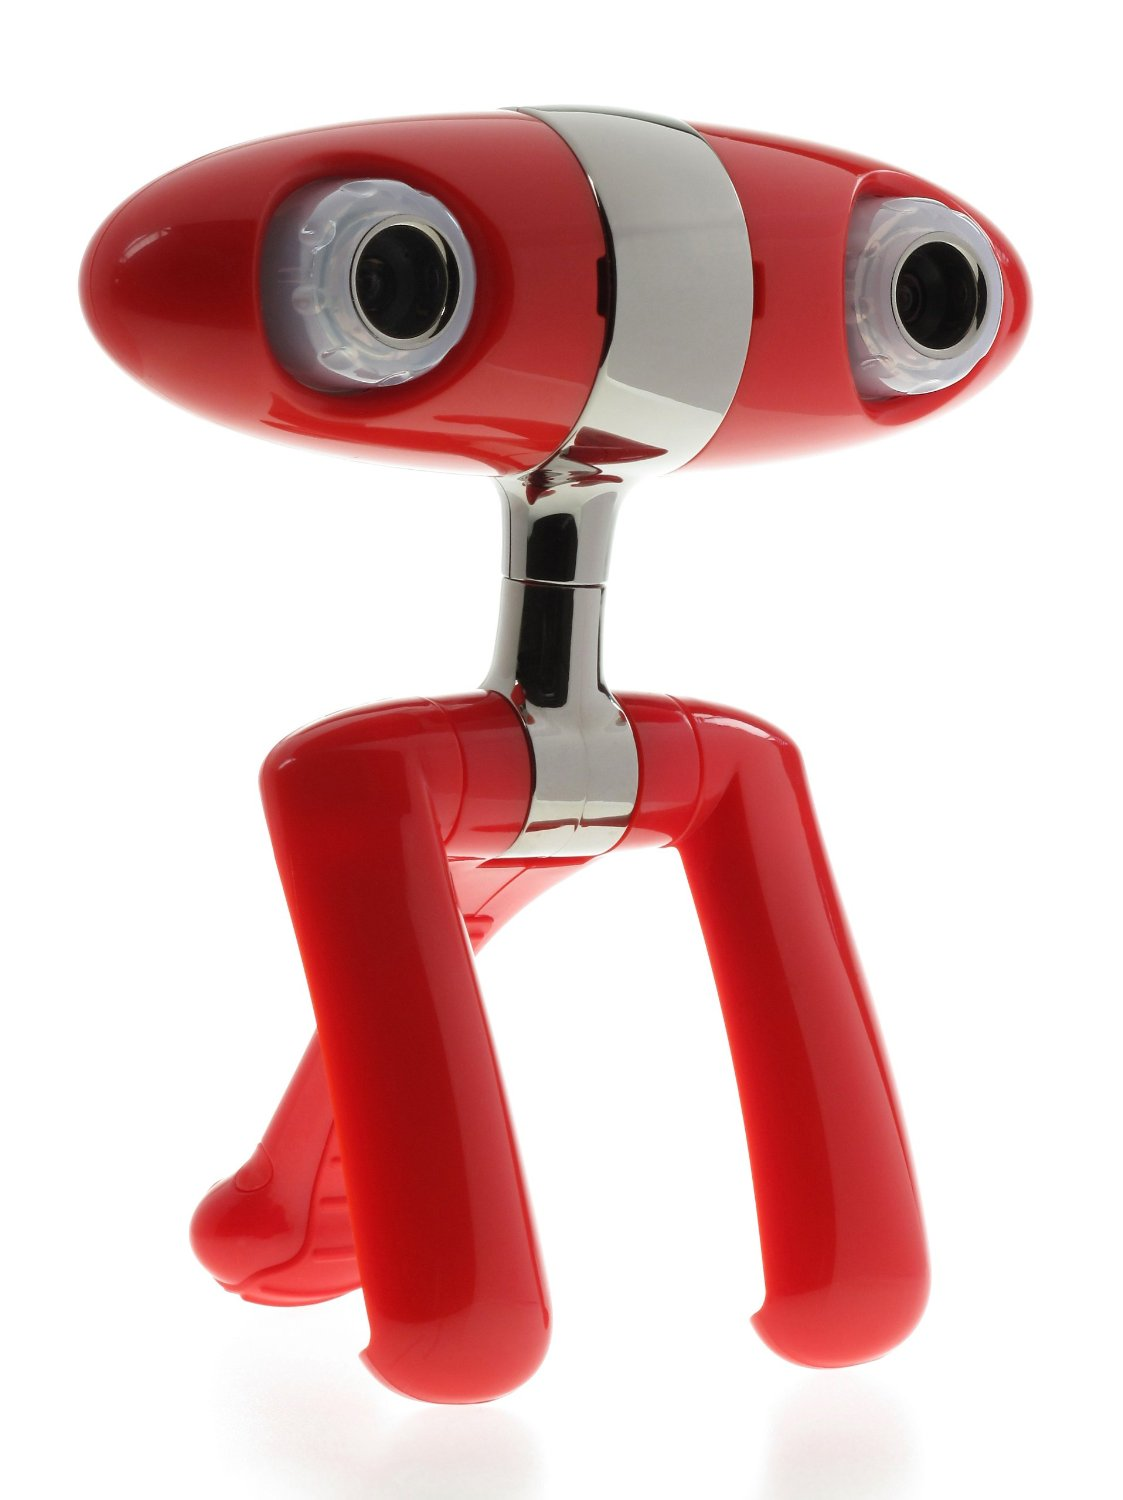
\includegraphics[scale=0.10]{./Resources/minoru.jpg}
	\caption{Fotografia da 3D Webcam Minoru}
	\label{minoru}
\end{figure}

\begin{table}[]
\centering
\caption{Especificações - 3D Webcam Minoru}
\label{minoru_tab}
\begin{tabular}{|c|c|}
\hline
\textbf{Sensor de Imagem}      & VGA CMOS Sensor  		\\	\hline
\textbf{Resolução Máxima}      & $800x600$        		\\	\hline
\textbf{Distância entre Sensores (\textit{Baseline})} & 6 cm    \\	\hline
\textbf{Taxa de Captura}       & 30 fps             		\\	\hline
\textbf{Distância Focal}       & 10 cm até $\infty$		\\	\hline
\textbf{Campo de Visão}        & $42\degree$			\\	\hline
\textbf{Peso}		       & 249.48 g			\\	\hline
\end{tabular}
\end{table}

Atualmente, a câmera utilizada é a digital 3D W3 fabricada pela Fujifilm (veja figura \ref{fujiW3}). A primeira câmera foi substituída, pois o controlador USB não permitia que a webcam realizasse \textit{streaming} na máxima resolução. Deste modo, optou-se por uma com maior resolução e que apresentasse lentes com baixa distorção. Entretanto, essa não apresenta \textit{streaming} via USB, assim é necessário que os vídeos sejam processados \textit{offline}. Visto que o projeto se preocupa principalmente na geração do mapa de disparidades, isso não oferece nenhuma desvantagem para o desenvolvimento do trabalho. Todavia, para uma aplicação real, a câmera instalada no veículo deve apresentar esse aspecto. A tabela \ref{fujiW3_tab} apresenta as especificações da câmera em questão.

\begin{table}[]
\centering
\caption{Especificações - Câmera Digital Fujifilm FinePix Real 3D W3}
\label{fujiW3_tab}
\begin{tabular}{|c|c|}
\hline
\textbf{Sensor de Imagem}      & 10 MP CCD Sensor  		\\	\hline
\textbf{Resolução Máxima}      & $1280x720$        		\\	\hline
\textbf{Distância entre Sensores (\textit{Baseline})} & 7.5 cm  \\	\hline
\textbf{Taxa de Captura}      & 24 - 30 fps          		\\	\hline
\textbf{Distância Focal}       & 60 cm até $\infty$		\\	\hline
\textbf{Peso}       		      & 250g			\\	\hline
\end{tabular}
\end{table}

\begin{figure}[H]
	\centering
	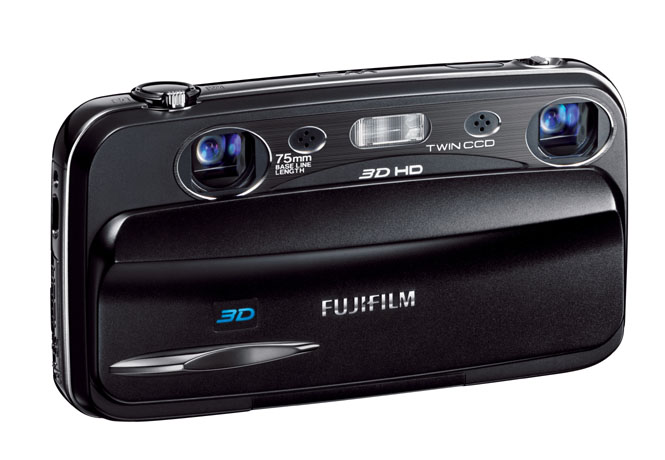
\includegraphics[scale=0.35]{./Resources/fujiW3.jpg}
	\caption{Fotografia da Câmera Digital Fujifilm FinePix Real 3D W3}
	\label{fujiW3}
\end{figure}


%-----------------------------------------------------------------------------------------------------------------------------------------------------------------------------------------------
\subsection{Unidades de Processamento}

Visto que este trabalho busca a implementação dos métodos estéreo em quadricópteros, tem-se como objetivo sua implementação para Linux embarcado (\textit{Embedded Linux}). Em seguida, estão apresentadas as plataformas que foram utilizadas para este propósito.


%-----------------------------------------------------------------------------------------------------------------------------------------------------------------------------------------------
\subsubsection{BeagleBone Black}

Uma das unidades de processamento utilizadas foi a plataforma aberta BeagleBone Black (BBB), ilustrada pela figura \ref{bbb}. Esta plataforma foi escolhida devido ao seu tamanho reduzido, podendo ser facilmente embarcada, isto é, é possível adaptá-la mecanicamente ao veículo. Com relação ao seu poder de processamento, ela apresenta um processador ARM Cortex-A8 operando à 1 GHz. A tabela \ref{bbb_tab} apresenta as especificações da plataforma.

\begin{table}[]
\centering
\caption{Especificações - BeagleBone Black}
\label{bbb_tab}
\begin{tabular}{|c|c|}
\hline
\textbf{Processador}           & 1GHz TI Sitara AM3359 ARM Cortex-A8			\\	\hline
\textbf{RAM}                   & 512 MB DDR3L à 400 MHz					\\	\hline
\textbf{Armazenamento}         & 2 GB on-board eMMC, MicroSD				\\	\hline
\textbf{Sistemas Operacionais} & Angstrom (Default), Ubuntu, Android, dentre outros...	\\	\hline
\textbf{Consumo de energia}    & 210-460 mA à 5V					\\	\hline
\textbf{Pinos de GPIO}         & 65/92 pinos						\\	\hline
\textbf{Periféricos}           & 1 USB Host, 1 Mini-USB Client, 1 10/100 Mbps Ethernet  \\	\hline                              
\end{tabular}
\end{table}

\begin{figure}[H]
	\centering
	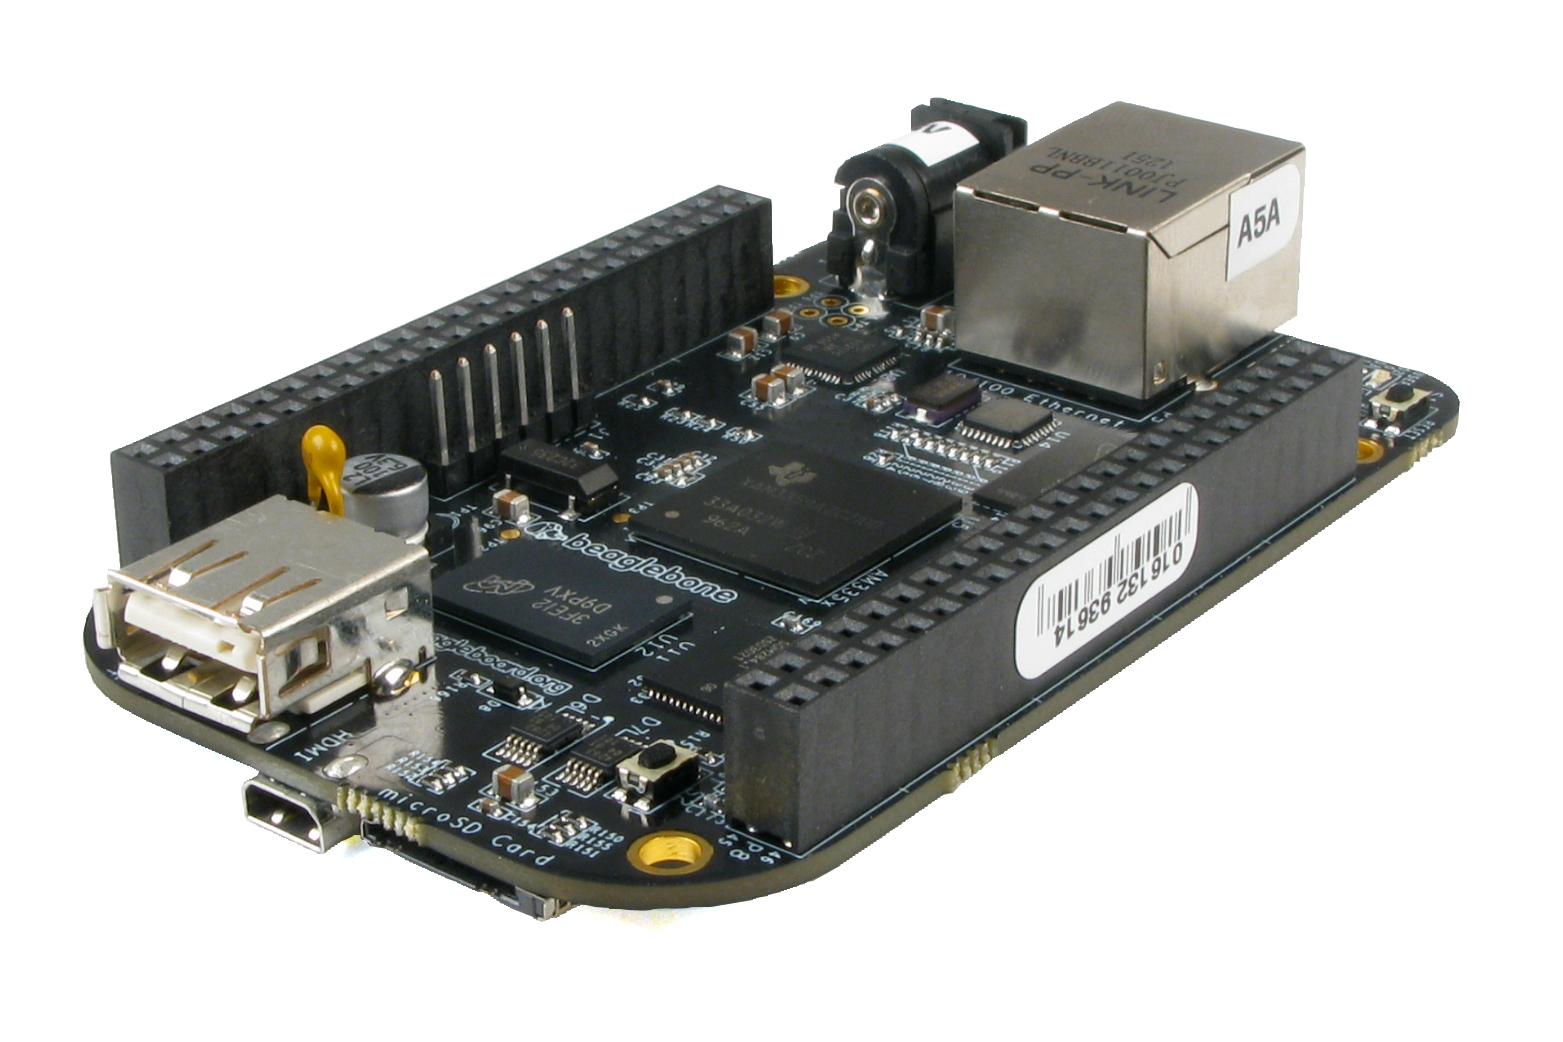
\includegraphics[scale=0.26]{./Resources/bbb.jpg}
	\caption{Fotografia da Plataforma de Desenvolvimento - BeagleBone Black}
	\label{bbb}
\end{figure}


%-----------------------------------------------------------------------------------------------------------------------------------------------------------------------------------------------
\subsubsection{Jetson TK1}

Outra unidade de processamento utilizada foi a plataforma \textit{Jetson TK1} produzida pela NVIDIA, ilustrada pela figura \ref{jetson_tk1}. Essa plataforma conta com um processador de 32-bits Tegra K1 baseado na tecnologia ARM Cortex-A15. O motivo pelo qual esta plataforma foi escolhida é devido ao seu poder de processamento gráfico, visto que apresenta 192 núcleos gráficos, sendo assim adequada para aplicações envolvendo processamento de imagens. A tabela \ref{jetson_tk1_tab} apresenta as especificações da plataforma. Outro fator interessante desta plataforma é que ela oferece suporte à tecnologia CUDA.

\begin{table}[]
\centering
\caption{Especificações - \textit{Jetson TK1}}
\label{jetson_tk1_tab}
\begin{tabular}{|c|c|}
\hline
\textbf{Processador}           & NVIDIA 2.32GHz ARM quad-core Cortex-A15			\\	\hline
\textbf{Processador Gráfico}   & NVIDIA Kepler "GK20a" GPU com 192 núcleos de CUDA SM3.2	\\	\hline
\textbf{DRAM}                  & 2GB DDR3L 933MHz EMC x16 usando largura de dados de 64-bit	\\	\hline
\textbf{Armazenamento}         & Memória de Armazenamento Rápido de 16GB eMMC 4.51		\\	\hline
\textbf{Sistemas Operacionais} & Plataforma Linux Ubuntu 14.04 64-bit                  		\\	\hline
\textbf{Consumo de energia}    & 0.6W à 3W à 12 V                    		\\	\hline
\textbf{Pinos de GPIO}         & 7 x pinos de GPIO (1.8V)                              		\\	\hline
\textbf{Periféricos}           & USB, mini-PCIe, SATA, SD-card, HDMI, Áudio           		\\	\hline
\end{tabular}
\end{table}

\begin{figure}[H]
	\centering
	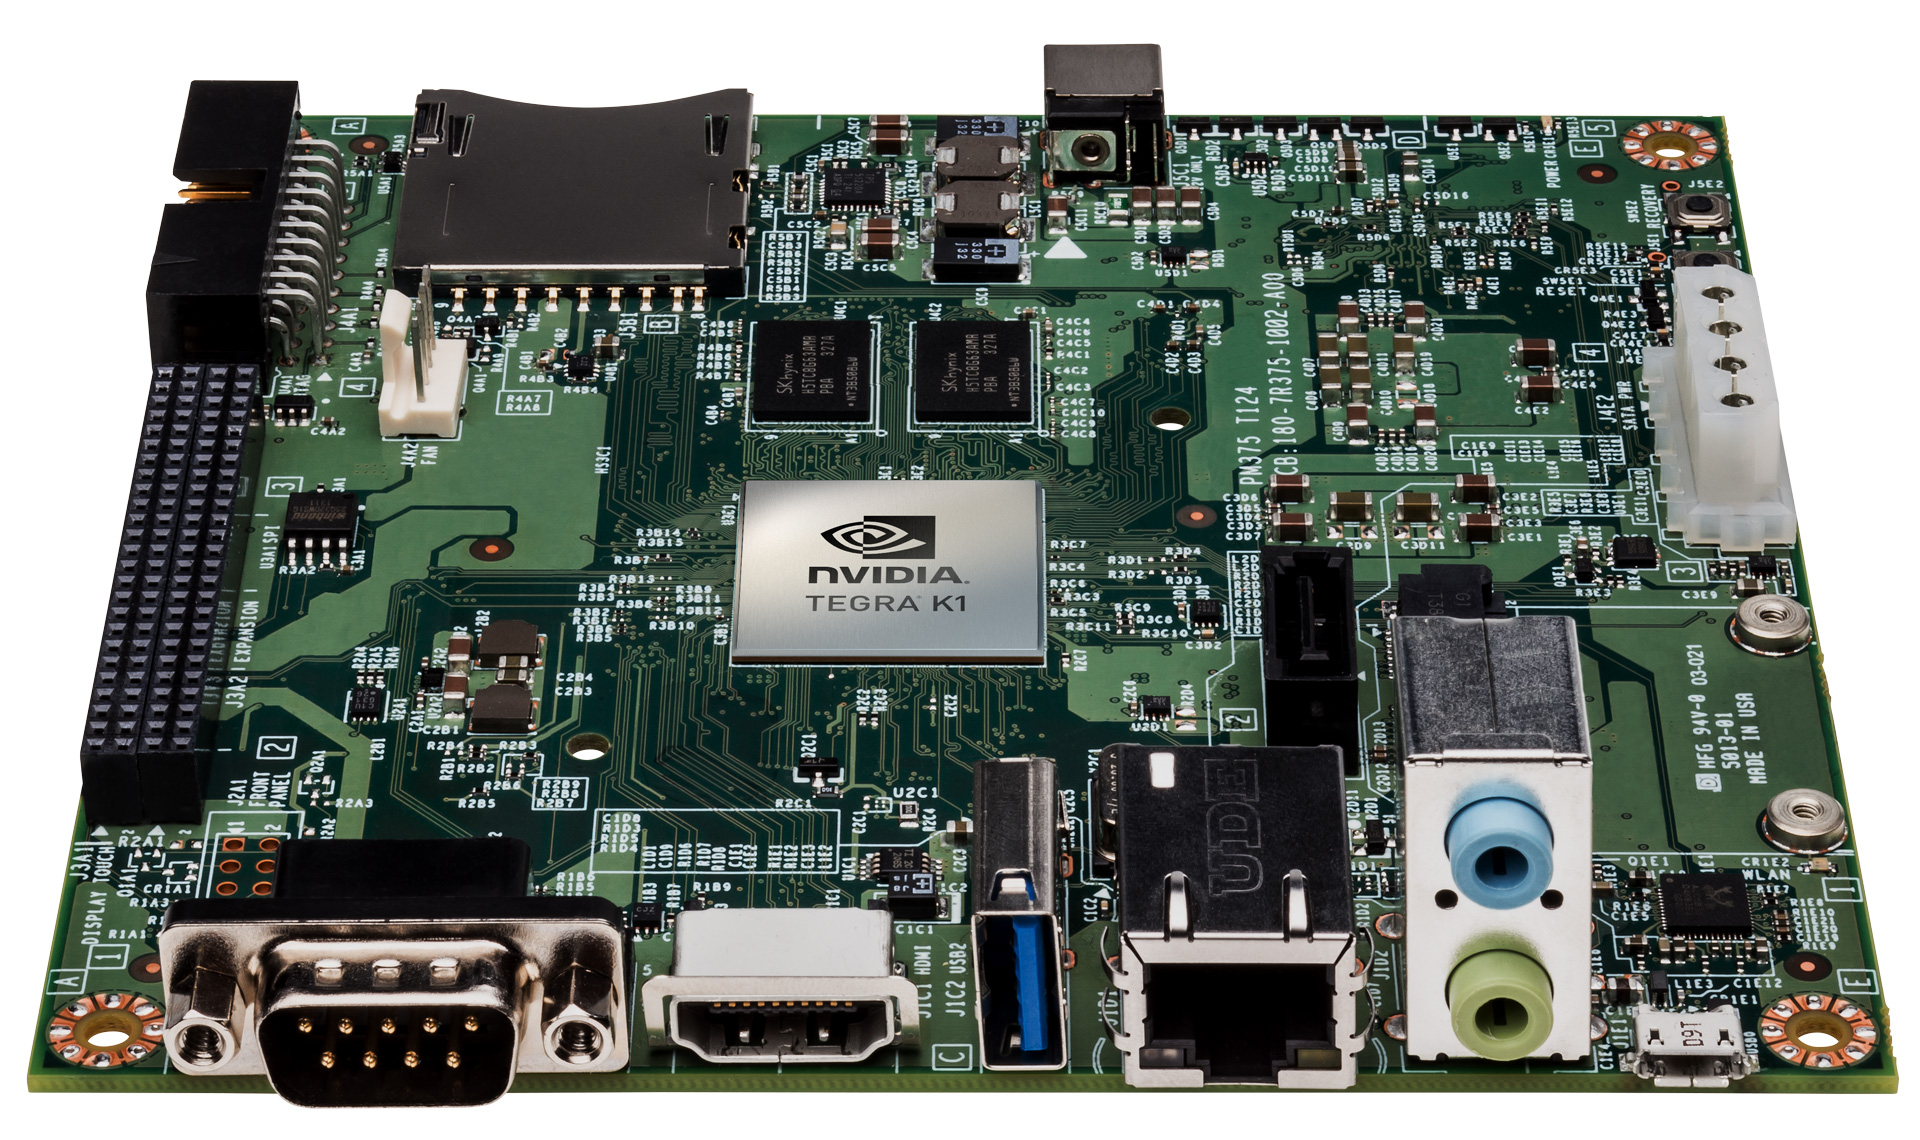
\includegraphics[scale=0.10]{./Resources/jetson_tk1.jpg}
	\caption{Fotografia da Plataforma de Desenvolvimento - \textit{Jetson TK1}}
	\label{jetson_tk1}
\end{figure}


%-----------------------------------------------------------------------------------------------------------------------------------------------------------------------------------------------
\subsubsection{Notebook Asus Q550LF}

Também foi utilizado um \textit{Notebook} Asus Q550LF, ele foi utilizada para o desenvolvimento de todos os programas contidos neste trabalho e para estudo de desempenho comparativo com as plataformas embarcadas. A interface desenvolvida, \textit{StereoVisionGUI}, foi desenvolvida para ser executada nesta máquina e em computadores com arquitetura x86 e x64. As especificações desta plataforma estão apresentadas pela tabela \ref{asusQ550LF}.

\begin{table}[]
\centering
\caption{Especificações - Asus Q550LF}
\label{asusQ550LF}
\begin{tabular}{|c|c|}
\hline
\multicolumn{2}{|c|}{\textbf{Especificações CPU}}                                                      		   \\ \hline
\textbf{Processador}             	& Intel Core i7 (Quarta Geração) 4500U / 1.8 $\sim$ 3.0 GHz           	   \\ \hline
\textbf{Número de Núcleos} 		& 2  	                                                                   \\ \hline
\textbf{Memória}          		& DDR3 SDRAM 8 GB                                                          \\ \hline
\multicolumn{2}{|c|}{\textbf{Especificações de GPU}}                                                   		   \\ \hline
\textbf{\textit{Chipset} da GPU}        & NVIDIA                                                      		   \\ \hline
\textbf{Arquitetura}    		& Kepler                                                                   \\ \hline
\textbf{Processador Gráfico}            & GK107 384 a 837 MHz                                         		   \\ \hline
\textbf{Memória da GPU}          	& DDR3 - 2048 MB - 128 Bit a 1800 MHz                                      \\ \hline
\textbf{Núcleos de CUDA}      		& 384 Núcleos                                                              \\ \hline
\textbf{Periféricos}        		& Optimus, GPU Boost 2.0, PhysX, Verde Drivers, CUDA, 3D Vision, 3DTV Play \\ \hline
\end{tabular}
\end{table}


%-----------------------------------------------------------------------------------------------------------------------------------------------------------------------------------------------
\subsection{Equipamentos auxiliares}

Nesta seção, estão apresentados os equipamentos auxiliares para o desenvolvimento do trabalho. 

Os métodos para a identificação de correspondências entre as câmeras requerem que as imagens estejam calibradas e retificadas. Por conta disso, utiliza-se o padrão de calibração de dimensão 7x10, apresentado na figura \ref{calibration_pattern}, para este propósito. Deste modo, é possível caracterizar as distorções das lentes, parâmetros intrínsecos, e o posicionamento de uma das câmeras com relação a outra, parâmetros extrínsecos.  

\begin{figure}[H]
	\centering
	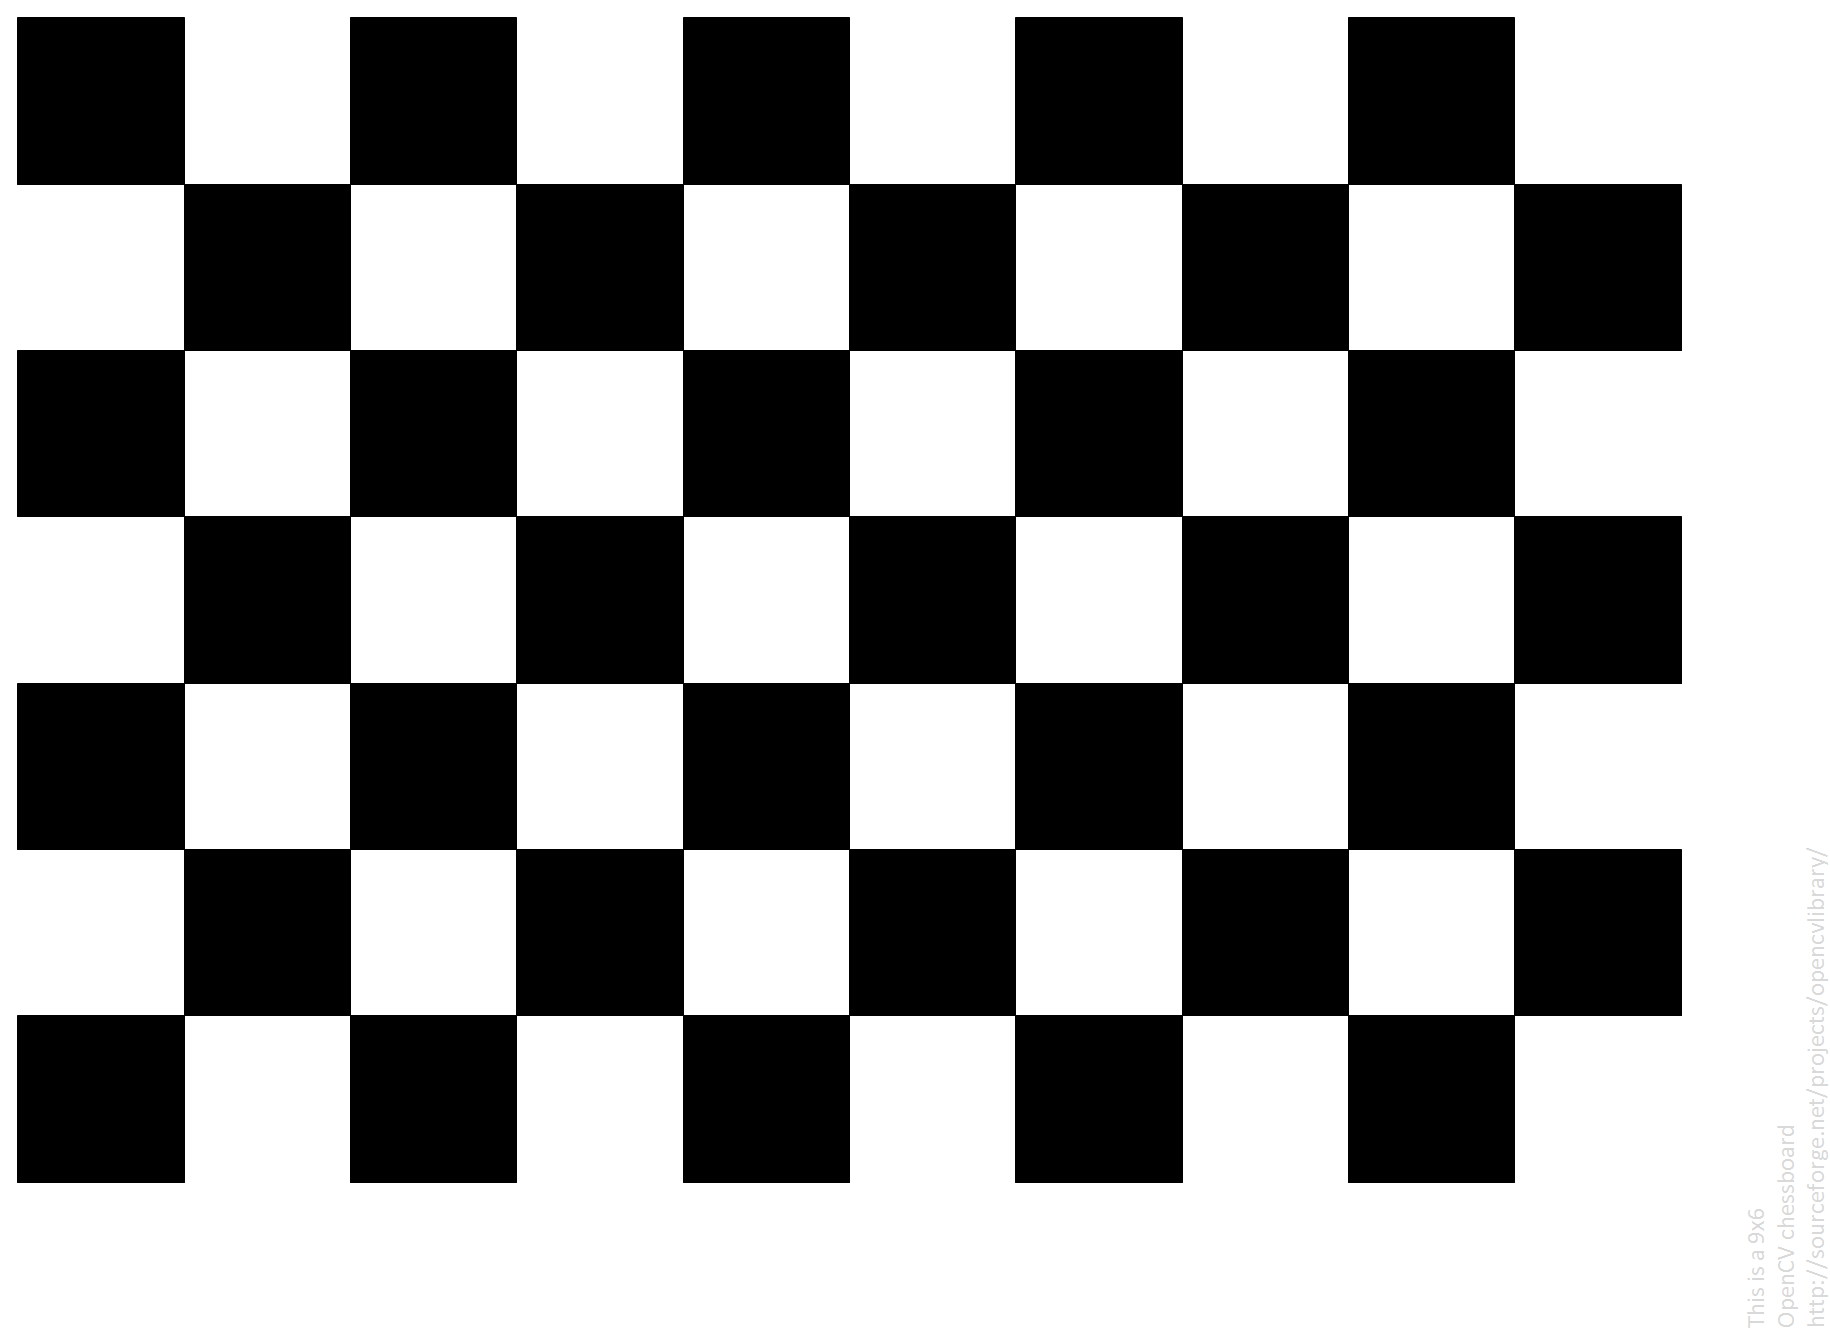
\includegraphics[scale=0.10]{./Resources/calibration_pattern.png}
	\caption{Fotografia do Padrão de Calibração}
	\label{calibration_pattern}
\end{figure}

A motivação deste trabalho é a sua utilização em veículos aéreos. Por conta disso, é indispensável que se tenha algum desses veículos. O trabalho conta com a utilização de um quadricóptero produzido pela 3DR\texttrademark \cite{3DRX8}, porém este apresenta modificações visando o seu desenvolvimento para navegação autônoma. Deste modo, tem-se a adição de \textit{propellers guards}, objetivando o aumento da segurança do veículo e das pessoas que o operam. Além disso, o \textit{drone} conta com suportes para a câmera estéreo e para a plataforma embarcada. Como pode ser observado na figura \ref{quad_camera_support}, todas as peças foram produzidas utilizando impressora 3D.

\begin{figure}[H]
	\centering
	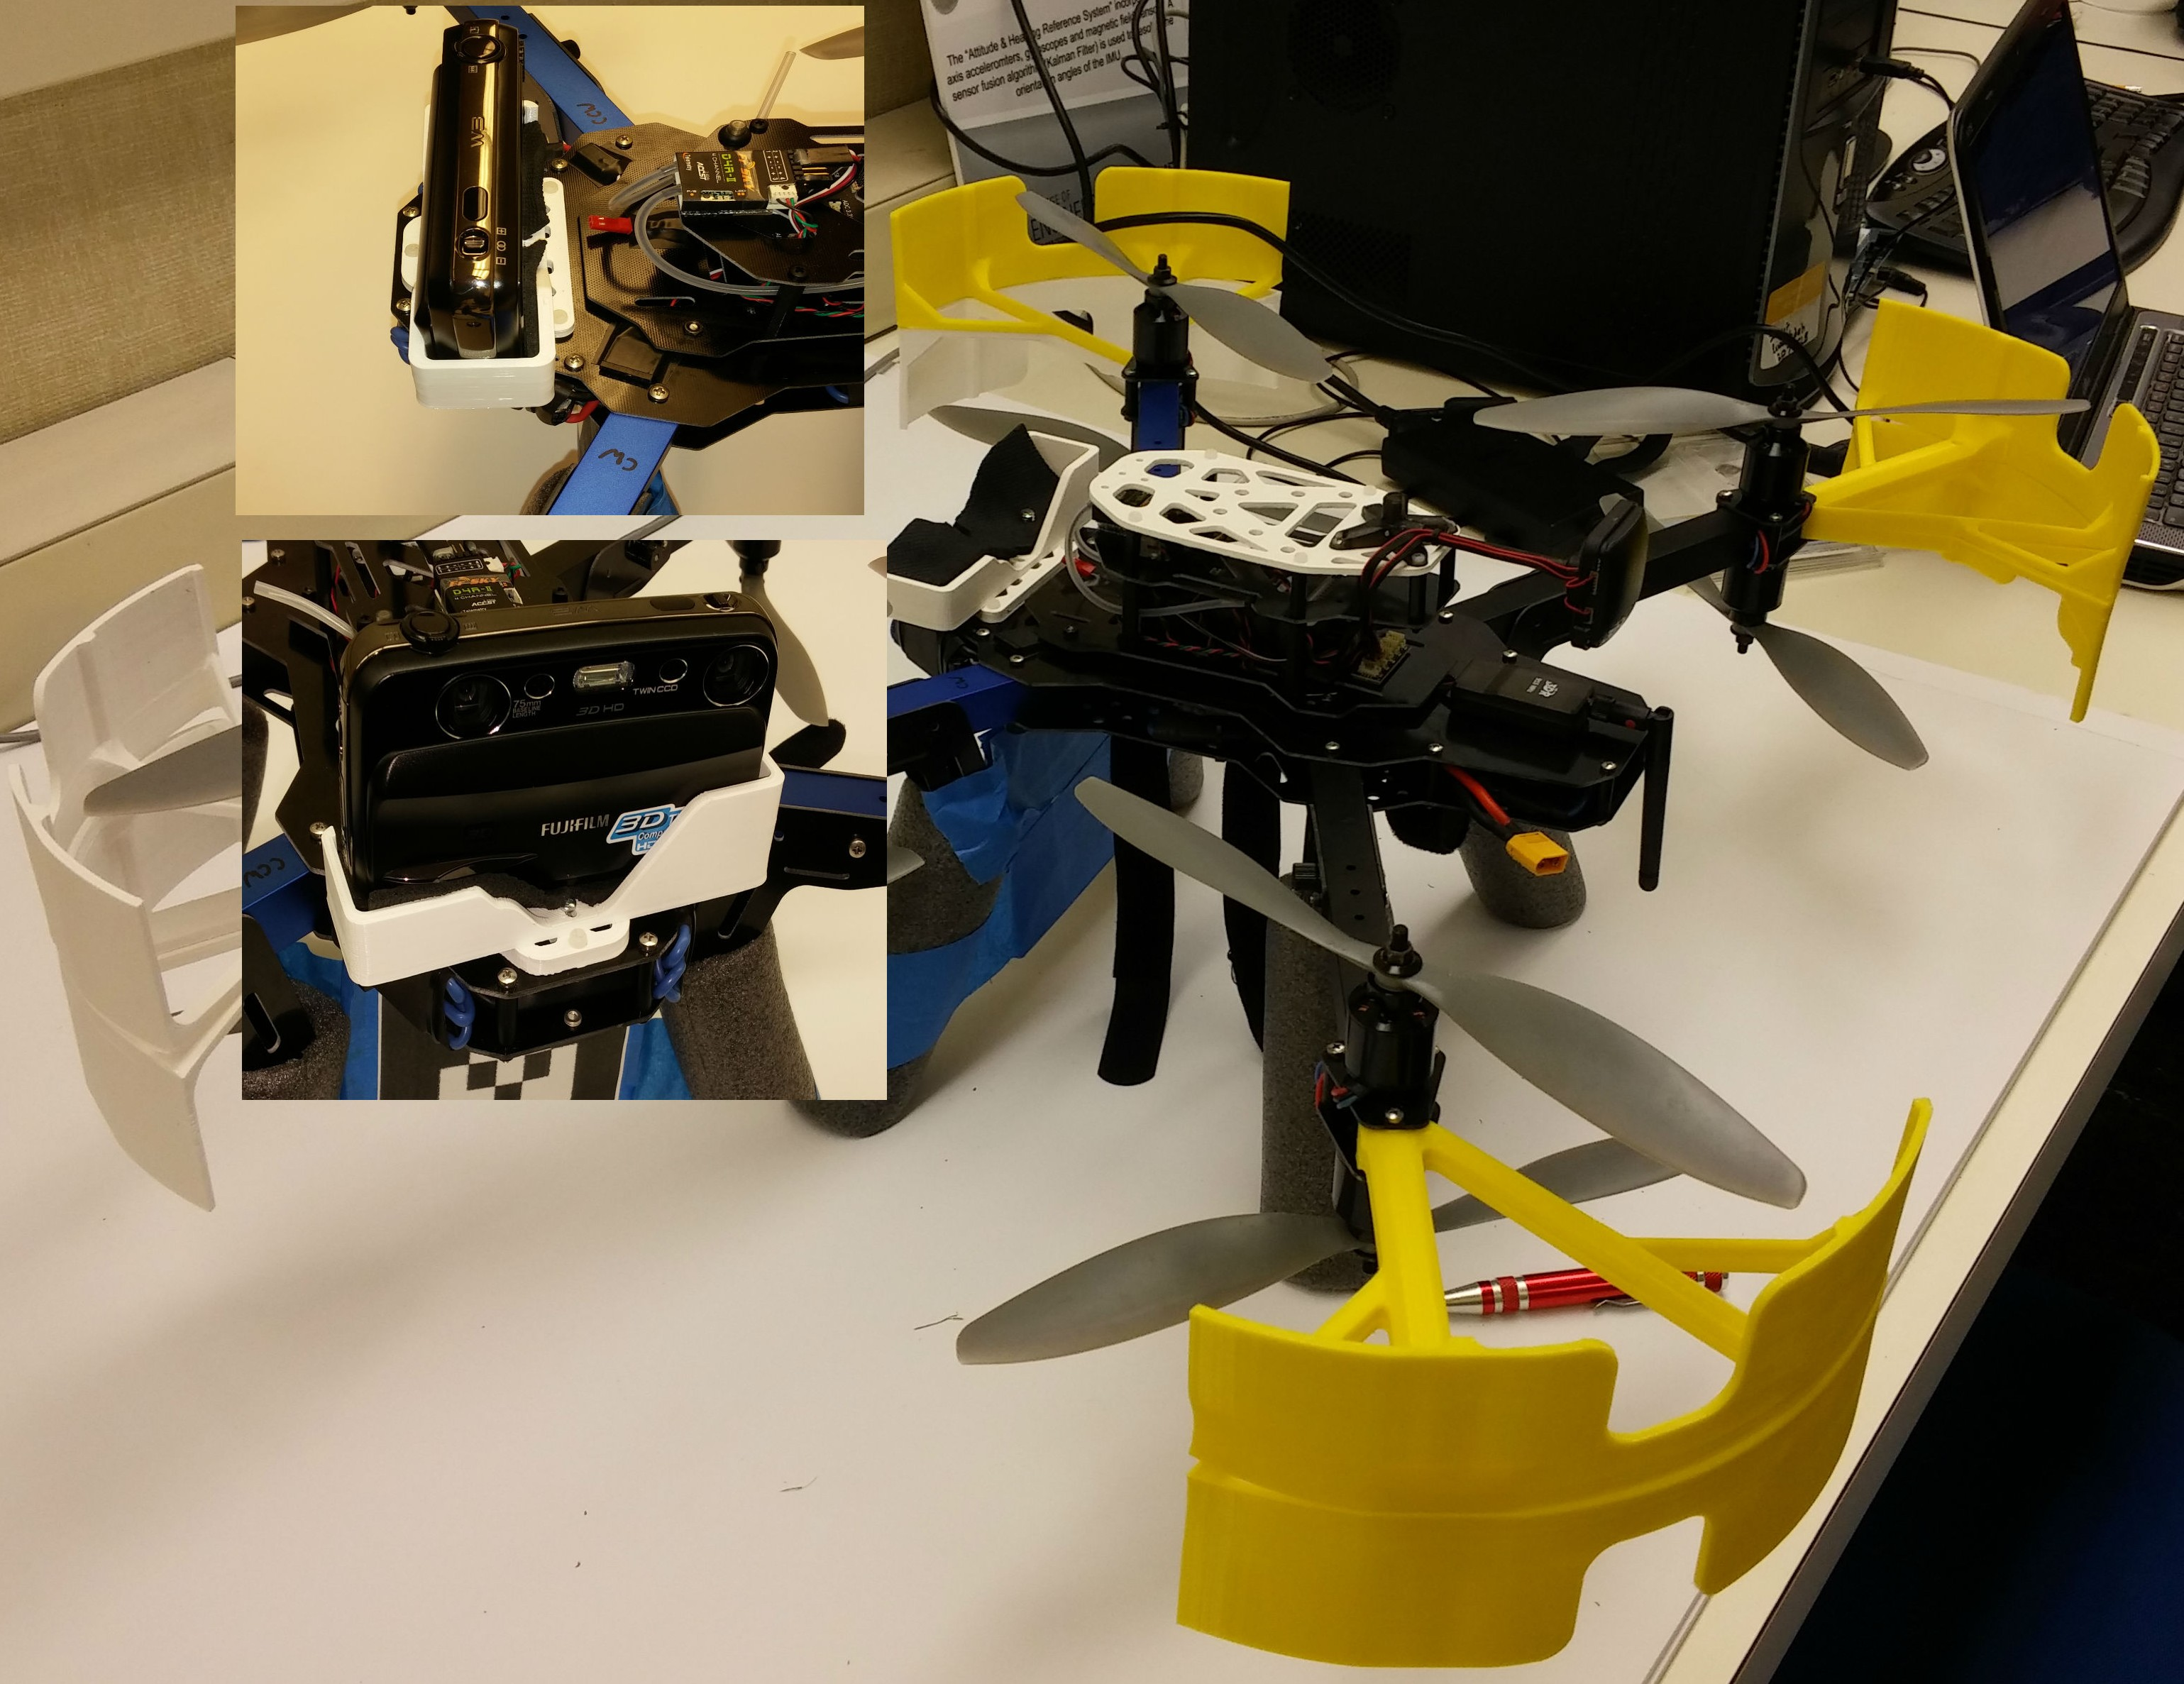
\includegraphics[scale=0.10]{./Resources/quad_camera_support.jpg}
	\caption{Fotografia do Quadricóptero 3DR X8 com suporte para a Câmera 3D}
	\label{quad_camera_support}
\end{figure}


%-----------------------------------------------------------------------------------------------------------------------------------------------------------------------------------------------
\section{Métodos}

Nesta seção, serão apresentados os cenários e os procedimentos utilizados na implementação dos métodos estéreo apresentados.


%-----------------------------------------------------------------------------------------------------------------------------------------------------------------------------------------------
\subsection{Cenários}
\label{scenes}

O pós-processamento do mapa de disparidades foi voltado para a identificação e detecção de obstáculos. Deste modo, os seguintes cenários propõem uma série de adversidades, as quais o algoritmo implementado tenta contorná-las. Propôs-se que ele deve ser flexível a variações na luminosidade, capaz de detectar obstáculos estáticos e móveis, e ser imune a vibrações. Deste modo, dois cenários em ambiente confinado e um em ambiente aberto foram analisados. Deseja-se a navegação autônoma ocorra até mesmo em casos que o sinal do Sistema de Posicionamento Global (GPS) seja perdido, por conta disso escolheu-se a utilização dos ambientes confinados. O ambiente externo foi escolhido devido a quantidade de fatores externos que poderiam atrapalhar a detecção de obstáculos. O tratamento destes percalços torna o programa ainda mais robusto.


%-----------------------------------------------------------------------------------------------------------------------------------------------------------------------------------------------
\subsubsection{Cenário 1}

O cenário da figura \ref{thumb_video10_l} foi utilizado para estudo das condições de ambiente externo, o qual está sujeito grandes variações de luminosidade e um número menor de movimentos, o que permite uma análise de alcances maiores. O principal  obstáculo deste cenário é uma árvore. 


%-----------------------------------------------------------------------------------------------------------------------------------------------------------------------------------------------
\subsubsection{Cenário 2}

O cenário da figura \ref{thumb_video12_l} foi utilizado para estudo das condições de ambiente interno, o qual também apresenta certa variação de luminosidade, porém apresenta um número maior de movimentos, permitindo uma análise de objetos estáticos à curta e média distância. Os principais obstáculos deste cenário são uma mesa, uma cadeira e duas estantes.


%-----------------------------------------------------------------------------------------------------------------------------------------------------------------------------------------------
\subsubsection{Cenário 3}

O cenário da figura \ref{thumb_video15} foi utilizado para estudo das condições de ambiente interno, o qual é semelhante ao cenário anterior com relação à luminosidade e o alcance analisado. A cena difere apenas na inserção de uma outra aeronave, a qual realiza o papel de um obstáculo móvel. Os principais obstáculos deste cenário é uma bancada e um outro quadricóptero no campo de visão do veículo pilotado.


%-----------------------------------------------------------------------------------------------------------------------------------------------------------------------------------------------
% Figuras
\begin{figure}[H]
	\centering
	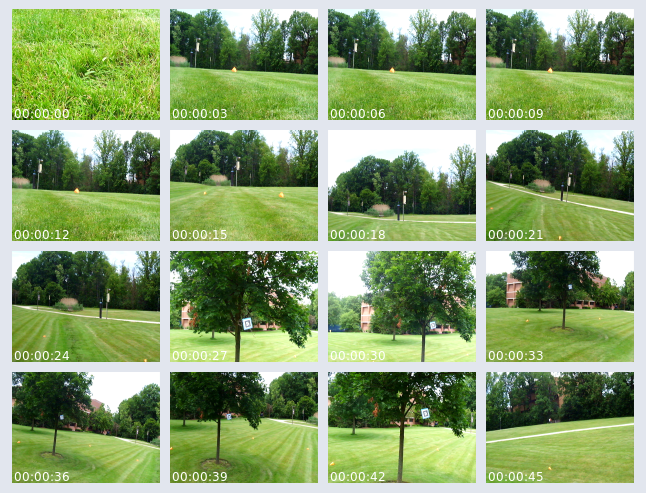
\includegraphics[scale=0.55]{./Resources/thumbs/thumb_video10_l.png}
	\caption{\textit{Thumbnail} do video referente ao Cenário 1 - Ambiente Externo - Árvore}
	\label{thumb_video10_l}
\end{figure}

\begin{figure}[H]
	\centering
	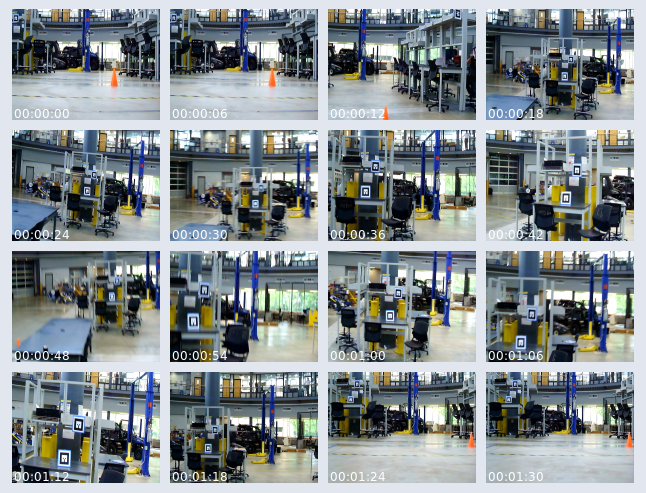
\includegraphics[scale=0.55]{./Resources/thumbs/thumb_video12_l.png}
	\caption{\textit{Thumbnail} do video referente ao Cenário 2 - Ambiente Interno - Mesa/Cadeira/Estantes}
	\label{thumb_video12_l}
\end{figure}

\begin{figure}[H]
	\centering
	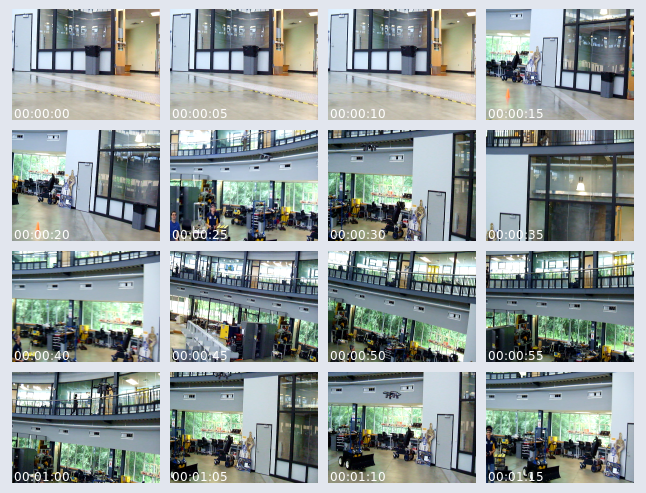
\includegraphics[scale=0.55]{./Resources/thumbs/thumb_video15.png}
	\caption{\textit{Thumbnail} do video referente ao Cenário 3 - Ambiente Interno - Bancada/Quadricóptero}
	\label{thumb_video15}
\end{figure}


%-----------------------------------------------------------------------------------------------------------------------------------------------------------------------------------------------
\subsection{Calibração}
O processo de calibração pode ser realizado em dois ambientes diferentes.  

O primeiro método é utilizando a rotina disponibilizada pelo OpenCV \cite{OpenCVCalibrationTutorial}, no qual algumas informações relevantes, como o tipo do padrão utilizado, o tamanho do padrão e o número de quadros, precisam ser informadas ao executá-la. Este método dispensa um conjunto de imagens de entrada para o processo de calibração, pois o próprio, automaticamente, se encarrega de detectar o padrão de calibragem e gravar as imagens utilizadas no processo. Ao fim da execução, as imagens são analisadas e os arquivos \textit{"intrinsics.yml"} e \textit{"extrinsics.yml"} são gerados, os quais contêm as matrizes que corrigem as distorções apresentadas na seção \ref{theory_calib}.

O segundo método é utilizando o aplicativo \textit{Stereo Camera Calibrator} presente no MATLAB. Ele também gera as mesmas informações anteriores, porém permite uma análise ainda mais profunda das distorções das lentes, como o erro de reprojeção 2D de cada imagem ou por pixel. Entretanto, é necessário que um conjunto de pares de imagens seja disponibilizado para o aplicativo para que a calibração seja realizada.

Os dois ambientes foram utilizados para efeito de validação dos parâmetros obtidos pelas calibrações.

%-----------------------------------------------------------------------------------------------------------------------------------------------------------------------------------------------
\subsubsection{Parâmetros intrínsecos}

O MATLAB disponibiliza gráficos que representam as distorções das ambas as lentes, assim como apresentado na imagem \ref{lenses_distortion}, na qual é possível visualizar três modelos de distorção das lentes. O primeiro par de imagens corresponde ao modelo de distorção completo de ambas as lentes e leva em consideração as distorções radiais e tangenciais. O segundo par de imagens é o modelo de distorção considerando apenas a componente radial. O último par ilustra o modelo de distoção que considera apenas a componente tangencial.

\begin{figure}[H]
 	\centering
 	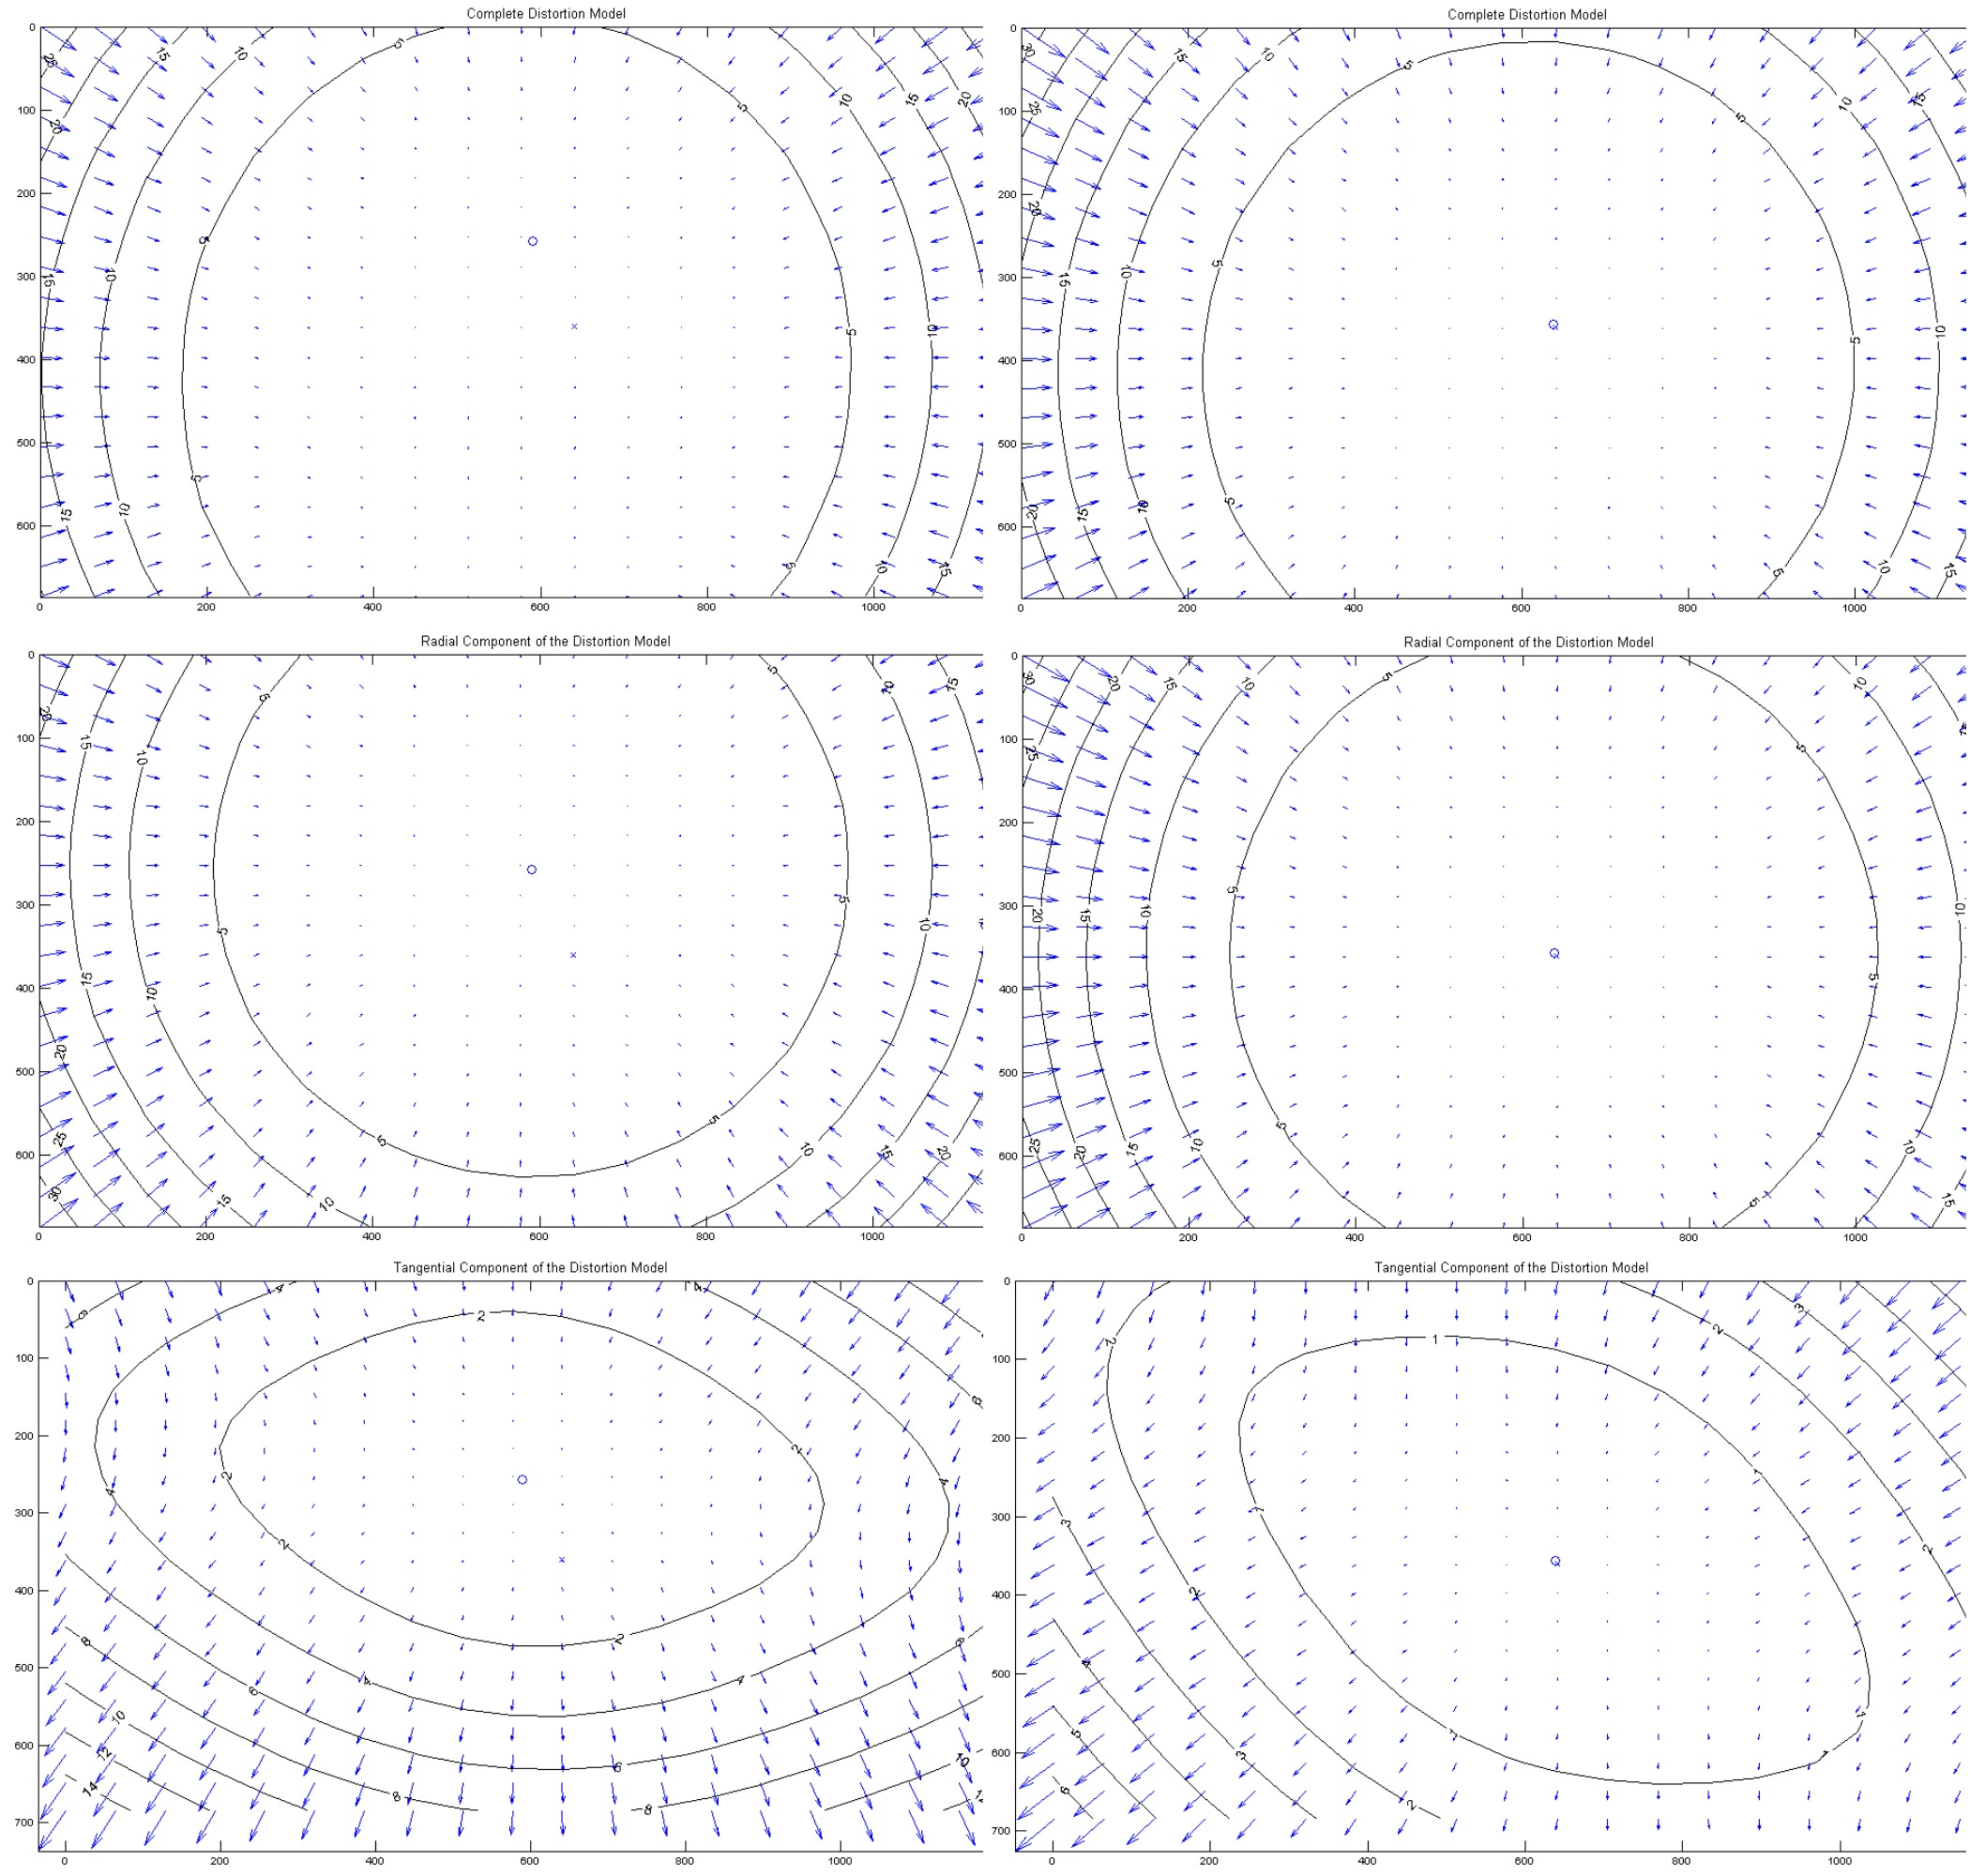
\includegraphics[scale=0.20]{./Resources/distortion/lenses_distortion.jpg}
 	\caption{Calibração estéreo dos parâmetros intrínsecos - Modelo de Distorções da câmera esquerda e direita, respectivamente. Imagem obtida utilizando \textit{Camera Calibration Toolbox for MATLAB} \cite{Bouguet1999}.}
 	\label{lenses_distortion}
\end{figure}


%-----------------------------------------------------------------------------------------------------------------------------------------------------------------------------------------------
\subsubsection{Parâmetros extrínsecos}

Como dito anteriormente, dado um conjunto de pares de imagens de um padrão de calibração é possível obter os parâmetros extrínsicos do equipamento estéreo. Além disso, também é possível estimar a reconstrução da cena utilizada no processo de calibração, onde estima-se o posicionamento de cada perspectiva das imagens utilizadas com relação às câmeras, assim como ilustrado na figura \ref{stereo_calib_extrinsic}. Ao fim do processo, são obtidos os parâmetros que descrevem a orientação da segunda câmera (Vermelha) em relação a primeira (Azul).

\begin{figure}[H]
 	\centering
 	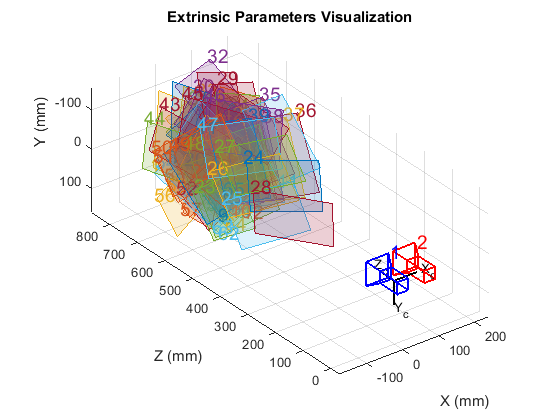
\includegraphics[scale=0.70]{./Resources/stereo_calib_extrinsic.png}
 	\caption{Calibração estéreo dos parâmetros extrínsecos - Estimativa do posicionamento da câmera direita$^2$ em relação à câmera esquerda$^1$. Imagem obtida utilizando o aplicativo \textit{Stereo Calibration App} do MATLAB \cite{MatlabStereoApp}.}
 	\label{stereo_calib_extrinsic}
\end{figure}

%-----------------------------------------------------------------------------------------------------------------------------------------------------------------------------------------------
\subsection{Processamento de Imagem}

Nessa seção será apresentado o processamento de imagens utilizado para a identificação de obstáculos. Como pode ser visto na figura \ref{stereo_processor_steps}, todo o processo conta com seis etapas.

\textbf{Câmeras:} O primeiro passo do processo é a captura das imagens da câmera estéreo. Idealmente, as imagens devem ser capturadas ao mesmo instante e as lentes não apresentarem distorções.   

\textbf{Calibração e Retificação:} Na prática, as lentes apresentam distorção. Com base nos parâmetros obtidos após a calibração das câmeras é possível retificá-las. 

\textbf{Correspondência Estéreo:} Aplica-se os métodos para encontrar as correspondências entre as duas câmeras, gerando assim o mapa de disparidades.

\textbf{Filtragem:} Este passo, pode ser aplicado tanto nas imagens retificados ou no mapa de disparidades. Atualmente, aplica-se a operação morfológica de abertura e um filtro de mediana sobre o mapa de disparidades. 

\textbf{Limiarização por Distância:} Visto que a disparidade apresenta uma relação com a distância, aplica-se uma operação de limiarização. Deste modo, apenas os obstáculos a uma certa distância são segmentados.

\textbf{Identificação de Obstáculos:} Após o passo anterior, o objeto é identificado e sua posição é rastreada. Essa informação pode ser utilizada pelo sistema de controle da aeronave para manter distância do obstáculo identificado. Esta etapa encontra-se realçada na figura \ref{stereo_processor_steps}, pois o processo de segmentação e identificação de objetos varia conforme o tipo de obstáculo e as condições da imagem (claro, escuro, muito brilho, baixo contraste). Deste modo, uma árvore de opções surge a partir deste processo, todos com o intuito de contornar as adversidades presentes no ambiente.

\begin{figure}[H]
	\centering
	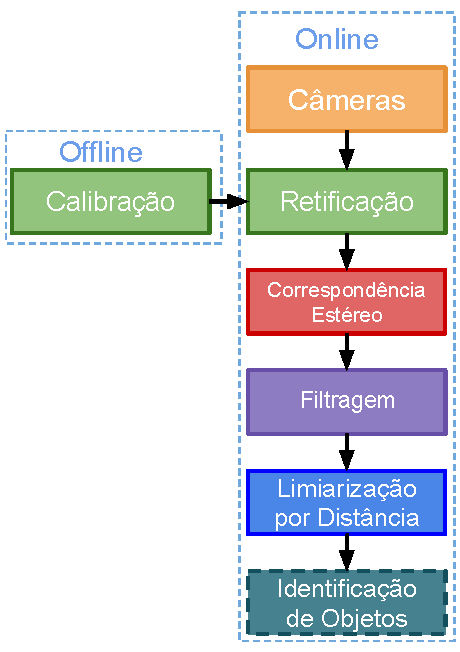
\includegraphics[scale=1.0]{./Resources/stereo_processor_steps3.pdf}
	\caption{Fluxograma do Processamento do Par de Imagens Estéreo}
	\label{stereo_processor_steps}
\end{figure}


%-----------------------------------------------------------------------------------------------------------------------------------------------------------------------------------------------
\subsection{Aceleração em Hardware - \textit{Hardware Acceleration} - CUDA}

Neste trabalho, utilizou-se diferentes versões desta API (\textit{Application Programming Interface}) para o desenvolvimento para \textit{Desktop} e \textit{Jetson TK1}. Neste contexto, essas versões não oferecem nenhuma alteração visível, visto que não foi desenvolvido nenhum tipo de rotina especificamente para execução em GPU. Na verdade, utilizou-se as funções disponíveis na biblioteca OpenCV, as quais opcionalmente podem ser executadas pela CPU ou GPU. A tabela \ref{cudaopencv} informa as versões do pacote de ferramentas da plataforma CUDA e da biblioteca OpenCV utilizadas. 

\begin{table}[]
\centering
\caption{Versões utilizadas de CUDA e OpenCV}
\label{cudaopencv}
\begin{tabular}{cccll}
                     & \textbf{CUDA ToolKit}	     & \textbf{OpenCV} 	       &  &  \\
\textbf{Desktop}     & 7.5                           & 3.0.0                   &  &  \\
\textbf{Jetson TK1}  & 6.5                           & 2.4.12                  &  &  \\
\multicolumn{1}{l}{} & \multicolumn{1}{l}{}          & \multicolumn{1}{l}{}    &  & 
\end{tabular}
\end{table}

\subsubsection{Desktop - Instalação e Configuração}
Abaixo, estão apresentadas as instruções necessárias para a instalação e a configuração do ambiente de desenvolvimento para que plataforma CUDA funcione corretamente \cite{FacebookCUDA}. O seguinte processo também pode ser executado para a configuração do ambiente na \textit{Jetson TK1}. Entretanto, um processo muito mais intuitivo e recomendado para essa plataforma está apresentado na seção \ref{jetsonSetupCUDA}.

\begin{enumerate}
 \item Instalando a CUDA
 
 Primeiramente, as seguintes instruções são compatíveis somente em máquinas com Ubuntu 14.04+ e com processadores gráficos da NVIDIA com capacidade de computação 3.5 ou maior. 
 \begin{enumerate}
  \item  Execute o seguinte comando:
  
\begin{lstlisting}[basicstyle=\tiny]
  $ ubuntu@ubuntu:~$ sudo apt-­get install build­-essential
\end{lstlisting}
  
Caso o usuário esteja utilizando uma máquina virtual, é necessário que os seguintes comandos sejam executados:

\begin{lstlisting}[basicstyle=\tiny]
  $ ubuntu@ubuntu:~$ sudo apt-get update
  $ ubuntu@ubuntu:~$ sudo apt-get install linux-generic
\end{lstlisting}

\item Baixe o arquivo .deb da CUDA no seguinte link: \url{https://developer.nvidia.com/cuda-downloads}, e verifique se a versão do arquivo é correspondente ao sistemas operacional utilizado. Neste trabalho, utilizou-se o Linux Ubuntu 14.04 64-bit e o arquivo condizente chamava-se "cuda-repo-ubuntu1404-7-5-local\_7.5-18\_amd64.deb" e foi possível instalá-lo recorrendo aos seguintes comandos:

\item Execute os seguintes comandos:

\begin{lstlisting}[basicstyle=\tiny]
$ ubuntu@ubuntu:~$ cd Downloads
$ ubuntu@ubuntu:~/Downloads$ sudo dpkg -i cuda-repo-ubuntu1404-7-5-local_7.5-18_amd64.deb
$ ubuntu@ubuntu:~/Downloads$ sudo apt-get update
$ ubuntu@ubuntu:~/Downloads$ sudo apt-get install cuda

\end{lstlisting}

\item Configure as variáveis do ambiente necessárias para o desenvolvimento em programação CUDA:
 
\begin{lstlisting}[basicstyle=\tiny]
$ ubuntu@ubuntu:~/Downloads$ nano ~/.bashrc

-----------------------------------------------------------------------
    Edite o arquivo /home/<user>/.bashrc e adicione o seguinte trecho:
-----------------------------------------------------------------------
# CUDA Environment Setup 
# CUDA 6.5
#export PATH=/usr/local/cuda-6.5/bin:$PATH
#export LD_LIBRARY_PATH=/usr/local/cuda-6.5/lib64:$LD_LIBRARY_PATH

# CUDA 7.5 (active)
export PATH=/usr/local/cuda-7.5/bin:$PATH
export LD_LIBRARY_PATH=/usr/local/cuda-7.5/lib64:$LD_LIBRARY_PATH

$ ubuntu@ubuntu:~/Downloads$ source ~/.bashrc
\end{lstlisting}

\item Reinicie o computador.
 \end{enumerate}

  \item Instalando do OpenCV com Suporte à CUDA \cite{Harasimowicz2015}
  \begin{enumerate}
   \item Instalando os pacotes necessários
   \begin{lstlisting}[basicstyle=\tiny]
$ ubuntu@ubuntu:~$ sudo apt-get update

$ ubuntu@ubuntu:~$ sudo apt-get install libopencv-dev build-essential checkinstall 
		   cmake pkg-config yasm libtiff4-dev libjpeg-dev libjasper-dev 
		   libavcodec-dev libavformat-dev libswscale-dev libdc1394-22-dev 
		   libxine-dev libgstreamer0.10-dev libgstreamer-plugins-base0.10-dev 
		   libv4l-dev python-dev python-numpy libtbb-dev libqt4-dev libgtk2.0-dev 
		   libfaac-dev libmp3lame-dev libopencore-amrnb-dev libopencore-amrwb-dev 
		   libtheora-dev libvorbis-dev libxvidcore-dev x264 v4l-utils
$ ubuntu@ubuntu:~$ sudo add-apt-repository ppa:jon-severinsson/ffmpeg  
$ ubuntu@ubuntu:~$ sudo apt-get update  
$ ubuntu@ubuntu:~$ sudo apt-get install ffmpeg  
$ ubuntu@ubuntu:~$ sudo apt-get install frei0r-plugins
   \end{lstlisting}

   \item Clonando o repositório do OpenCV. Neste trabalho, utilizou-se a versão 3.0.0:
   \begin{lstlisting}[basicstyle=\tiny]
$ ubuntu@ubuntu:~$ mkdir OpenCV  
$ ubuntu@ubuntu:~$ cd OpenCV
$ ubuntu@ubuntu:~/OpenCV$ git clone https://github.com/Itseez/opencv.git  
   \end{lstlisting}


   \item Instalando e realizando o \textit{build} da biblioteca OpenCV. Este passo é de extrema importância, pois é aqui que configura-se o OpenCV para dar suporte à CUDA. Certifique-se que a arquitetura de GPU configurada na \textit{flag} CUDA\_GENERATION corresponda realmente a da sua plataforma:
   \begin{lstlisting}[basicstyle=\tiny]
$ ubuntu@ubuntu:~/OpenCV$ mkdir build && cd build
$ ubuntu@ubuntu:~/OpenCV/build$ cmake -D CMAKE_BUILD_TYPE=RELEASE -D CMAKE_INSTALL_PREFIX=/usr/local 
-D WITH_TBB=ON -D WITH_V4L=ON -D INSTALL_C_EXAMPLES=ON -D INSTALL_PYTHON_EXAMPLES=ON -D BUILD_EXAMPLES=ON 
-D WITH_QT=ON -D WITH_OPENGL=ON -D ENABLE_FAST_MATH=1 -D CUDA_FAST_MATH=1 -D WITH_CUBLAS=1 -D CUDA_GENERATION=Kepler ..
$ ubuntu@ubuntu:~/OpenCV/build$ make -j4
$ ubuntu@ubuntu:~/OpenCV/build$ sudo make install
    \end{lstlisting}

   \item Configurando o \textit{LIBRARY SEARCH PATH}:
   \begin{lstlisting}[basicstyle=\tiny]
$ ubuntu@ubuntu:~/$ sudo sh -c 'echo "/usr/local/lib" > /etc/ld.so.conf.d/opencv.conf'
$ ubuntu@ubuntu:~/$ sudo ldconfig

  \end{lstlisting}

  \end{enumerate}

\end{enumerate}

%-----------------------------------------------------------------------------------------------------------------------------------------------------------------------------------------------
\subsection{Jetson TK1 - Configuração da Plataforma}
\label{jetsonSetupCUDA}

A execução das rotinas de visão estéreo com aceleração via GPU requisitam que a plataforma de desenvolvimento esteja corretamente configurada. Abaixo, encontra-se o tutorial para configurá-la para a operação desejada, isto é, basicamente, configurá-la para o correto funcionamento da CUDA e do OpenCV2. 

\begin{enumerate}
  \item Baixando o JetPack L4T
    \begin{enumerate}
      \item Clique \href{http://docs.nvidia.com/jetpack-l4t/index.html#developertools/mobile/jetpack/jetpack_l4t/2.1/jetpack_l4t_install.htm}{aqui} para ir ser redirecionado para a página do pacote de desenvolvimento Jetpack L4T. Caso o link esteja quebrado, vá até a página da NVIDIA e procure pela localização correta do pacote.  

      \item Na máquina \textit{Host} rodando Ubuntu, crie um novo diretório para armazenar os pacotes de instalação utilizando as seguintes linhas de comando.

      \begin{lstlisting}[basicstyle=\tiny]
	$ ubuntu@ubuntu:~$ mkdir flash
	$ ubuntu@ubuntu:~$ cd flash
	$ ubuntu@ubuntu:~/flash$ 
      \end{lstlisting}

      Uma ação importante que merece destaque é baixar o arquivo JetPack-\${VERSION}.run dentro do diretório criado (o caminho NÃO DEVE conter espaços).

      \item Dê permissão de execução para o arquivo baixado. 
      \begin{lstlisting}[basicstyle=\tiny]
	$ ubuntu@ubuntu:~/flash$ chmod +x JetPack-${VERSION}.run
	$ ubuntu@ubuntu:~/flash$ ./JetPack-${VERSION}.run
      \end{lstlisting}


    \end{enumerate}
  \item Instalando o JetPack L4T

    Siga as instruções no manual de usuário do kit de desenvolvimento da \textit{Jetson TK1}
    \begin{enumerate}
      \item Baixe o guia de instruções no seguinte link e clique na aba "\textit{Install Guide}". Link: \url{https://developer.nvidia.com/embedded/jetpack}
      \item Siga as instruções do instalador do Jetpack L4T.

      Uma informação que merece destaque é que o computador \textit{Host} e o dispositivo alvo (\textit{Jetson TK1}) DEVEM estar conectados à mesma rede. Isso pode ser feito conectando:
      \begin{enumerate}
	\item Máquina \textit{Host} e dispositivo alvo à mesma Intranet, no caso o dispositivo alvo tenha um endereço IP estático.
	\begin{lstlisting}[basicstyle=\tiny]
	    ----------------------------------------------------
	    Edite o /etc/network/interfaces:
	    ----------------------------------------------------    
	    auto lo
	    iface lo inet loopback
	    auto eth0
	    iface eth0 inet static
	    address 10.235.0.133
	    netmask 255.255.252.0
	    network 10.235.3.0
	    gateway 10.235.0.1
	    pre-up ifconfig eth0 hw ether 00:01:02:03:05:09
	    dns-nameservers  143.107.225.6 143.107.182.2 8.8.8.8
	 \end{lstlisting}

	 \item Máquina \textit{Host} e dispositivo alvo ao mesmo roteador. Neste caso, o dispositivo alvo DEVE ser capaz de encontrar o endereço IP por protocolo DHCP.
	 \begin{lstlisting}[basicstyle=\tiny]
	    ----------------------------------------------------
	    Edite o /etc/network/interfaces:
	    ----------------------------------------------------    
	    auto eth0
	    allow-hotplug eth0
	    iface eth0 inet dhcp
	 \end{lstlisting}
      \end{enumerate}


    \end{enumerate}
  \item Instalando o OpenCV com Módulo GPU na \textit{Jetson TK1}

  Primeiramente, deve-se baixar e instalar o pacote de ferramentas CUDA, uma vez que é necessário para OpenCV. Cabe ao usuário decidir se deseja se utilizar a biblioteca pré-compilada ou compilar a biblioteca do código-fonte. A primeira opção é a mais recomendada, visto que a biblioteca pré-compilada é a OpenCV4Tegra, uma versão otimizada em CPU e GPU do OpenCV para a \textit{Jetson TK1}. A segunda opção é recomendada caso deseja-se adicionar módulos que não estão presentes na versão OpenCV4Tetra \cite{eLinuxJetsonOpenCV}. 

\end{enumerate}
